% ======================================================================
% RStudio Presentation: Sensor Data Analysis and Machine Learning Example
% Author: Anatolie Jentimir
% Date: October 28, 2025
% ======================================================================
\documentclass[12pt]{article}
\usepackage{graphicx}
\usepackage{booktabs}
\usepackage{geometry}
\usepackage{hyperref}
\usepackage{fancyhdr}
\usepackage{amsmath}
\usepackage{listings}
\usepackage{xcolor}
\geometry{margin=1in}
\pagestyle{fancy}
\lhead{RStudio Presentation}
\rhead{Sensor Data Analysis}

\definecolor{rblue}{rgb}{0.13,0.27,0.54}
\lstset{
  language=R,
  basicstyle=\ttfamily\small,
  keywordstyle=\color{rblue}\bfseries,
  commentstyle=\color{gray},
  stringstyle=\color{orange},
  frame=single,
  breaklines=true,
  showstringspaces=false,
  columns=fullflexible
}

\begin{document}

\begin{center}
  {\LARGE \textbf{RStudio Presentation and Workflow Guide}}\\[6pt]
  {\large Sensor Data Analysis using Sensor\_Data.csv and Machine Learning (lm)}\\[2pt]
  {\normalsize Author: Anatolie Jentimir, STEM Club — Bunker Hill Community College}
\end{center}

\vspace{1em}

\section*{Objective}
This guide demonstrates how to use RStudio to import sensor data, summarize it, visualize relationships, and apply a simple machine learning model (linear regression using \texttt{lm()}) to predict sensor readings. The document serves both as a presentation and an instructional manual for students and STEM Club members.

\section{Environment Setup}
\subsection{Installing and Loading Packages}
Open RStudio and execute the following lines in the console:

\begin{lstlisting}
install.packages(c("tidyverse", "lubridate", "janitor", "caret"))
library(tidyverse)
library(lubridate)
library(janitor)
library(caret)
\end{lstlisting}

These packages provide tools for data cleaning, visualization, and machine learning.

\subsection{Folder Structure}
Recommended project layout:
\begin{itemize}
  \item \texttt{data/} — place \texttt{Sensor\_Data.csv}
  \item \texttt{R/} — contains analysis scripts
  \item \texttt{figs/} — stores generated plots
  \item \texttt{reports/} — output documents or summaries
\end{itemize}

\section{Importing the Dataset}
Place your CSV file in the \texttt{data/} directory and load it:

\begin{lstlisting}
path <- file.path("data", "Sensor_Data.csv")
df <- read_csv(path) %>% janitor::clean_names()

# Quick inspection
glimpse(df)
summary(df)
\end{lstlisting}

\paragraph{Tip:} \texttt{clean\_names()} standardizes headers (e.g., converts \texttt{Temperature (C)} to \texttt{temperature\_c}).

\section{Descriptive Statistics}
Compute the \textbf{sum}, \textbf{mean}, and \textbf{median} for each numeric column. If a timestamp column exists, the median date is also computed.

\begin{lstlisting}
num_cols <- df %>% select(where(is.numeric))

summary_tbl <- num_cols %>%
  summarise(across(everything(), list(
    sum = ~sum(.x, na.rm = TRUE),
    mean = ~mean(.x, na.rm = TRUE),
    median = ~median(.x, na.rm = TRUE)
  )))
print(summary_tbl)

# Median timestamp if present
maybe_time <- df %>% select(matches("time|date|timestamp|datetime"))
if (ncol(maybe_time) > 0) {
  tcol <- names(maybe_time)[1]
  tvec <- parse_date_time(df[[tcol]], orders = c("Ymd HMS", "mdY HM", "mdY"))
  med_time <- median(as.numeric(tvec), na.rm = TRUE) %>%
    as.POSIXct(origin = "1970-01-01", tz = "UTC")
  print(med_time)
}
\end{lstlisting}

\section{Visualization}
We create a scatter plot to explore the correlation between two key sensor measurements (e.g., temperature and humidity):

\begin{lstlisting}
ggplot(df, aes(x = temperature, y = humidity)) +
  geom_point(color = "blue") +
  geom_smooth(method = "lm", col = "red") +
  theme_minimal() +
  labs(title = "Temperature vs Humidity", x = "Temperature", y = "Humidity")
\end{lstlisting}

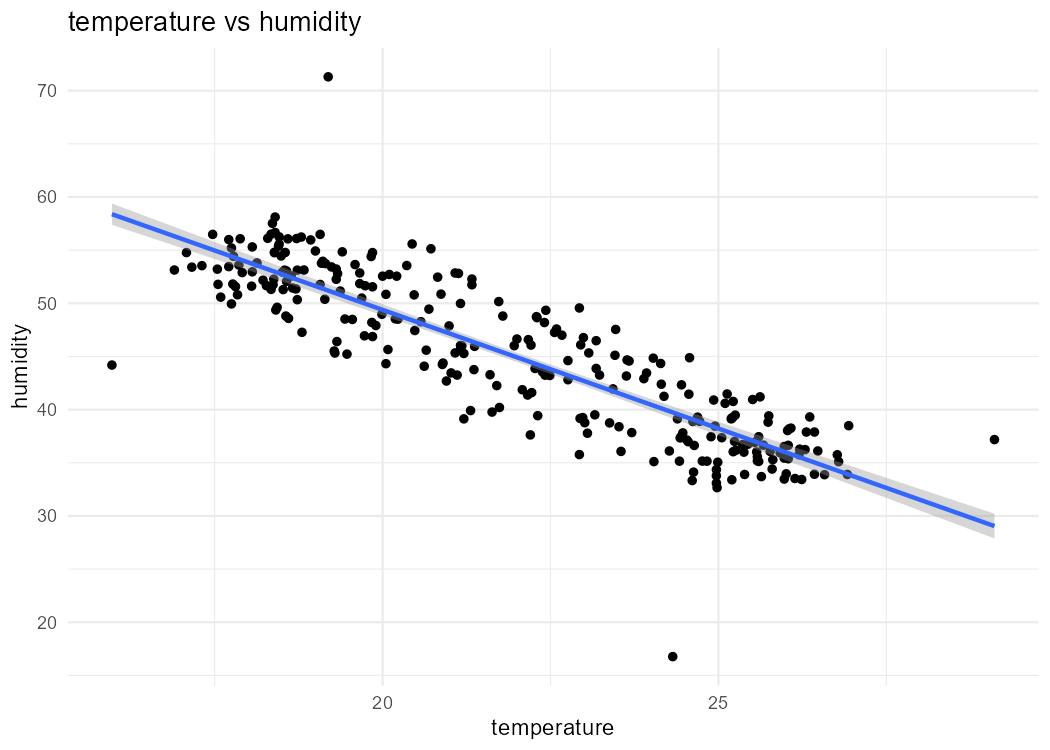
\includegraphics[width=0.8\textwidth]{figs/temperature_vs_humidity.png}

\section{Linear Regression (Machine Learning Model)}
We apply the linear model function \texttt{lm()} to predict humidity from temperature or other predictors.

\begin{lstlisting}
model <- lm(humidity ~ temperature, data = df)
summary(model)

df$predicted <- predict(model, df)

RMSE <- sqrt(mean((df$humidity - df$predicted)^2))
R2 <- cor(df$humidity, df$predicted)^2
cat("RMSE:", RMSE, "R²:", R2)
\end{lstlisting}

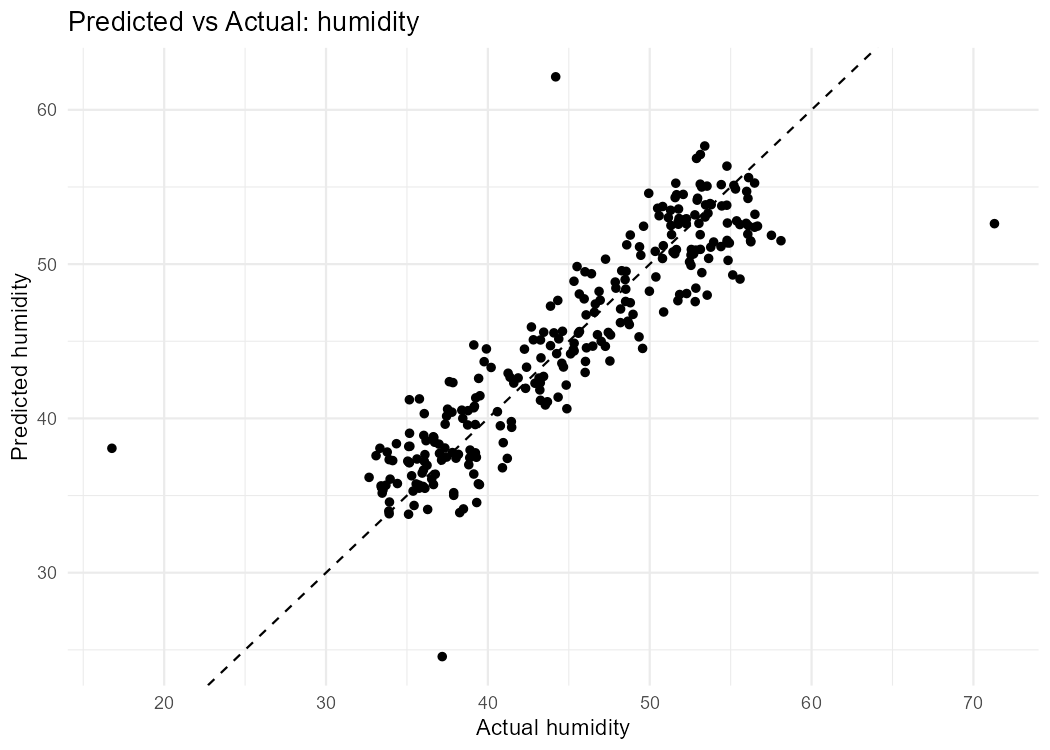
\includegraphics[width=0.8\textwidth]{figs/pred_vs_actual_humidity.png}

\section{Saving Visual Outputs}
You can save the generated plots for reports or web dashboards:

\begin{lstlisting}
# Save the last plot
if(!dir.exists("figs")) dir.create("figs")

ggsave("figs/temp_vs_humidity.png", width = 7, height = 5, dpi = 150)
\end{lstlisting}

\section{RStudio Shortcuts}
\begin{center}
\begin{tabular}{ll}
\toprule
\textbf{Action} & \textbf{Shortcut} \\
\midrule
Run selected code & Ctrl + Enter \\
Insert assignment operator (\texttt{<-}) & Alt + - \\
Comment / Uncomment line & Ctrl + Shift + C \\
Run all code chunks & Ctrl + Alt + R \\
Reformat code & Ctrl + Shift + A \\
Find in file & Ctrl + F \\
\bottomrule
\end{tabular}
\end{center}

\section{Common Issues}
\begin{itemize}
  \item Ensure columns used in \texttt{lm()} are numeric.
  \item Remove or impute missing values with \texttt{na.omit()}.
  \item Use \texttt{clean\_names()} to avoid spaces or special characters in column names.
  \item Verify the correct date format before parsing.
\end{itemize}

\section{Next Steps}
\begin{itemize}
  \item Extend the model with multiple predictors: \texttt{lm(humidity ~ temperature + soil\_moisture)}.
  \item Explore machine learning packages: \texttt{randomForest}, \texttt{xgboost}, or \texttt{caret::train()}.
  \item Automate periodic analysis using \texttt{R Markdown} or \texttt{knitr}.
\end{itemize}

\vfill
\noindent\textit{Prepared for:} STEM Club — Bunker Hill Community College \\
\textit{Author:} Anatolie Jentimir (2025)

\end{document}
